\subsection{Device Operations}
\label{sec:readwrite}
There are two operations that are issued by the driver --- read and write.
In order to perform these commands, the driver keeps track of the most 
recent version for each replica in a list, essentially acting as the master
for the system. This replica versioning structure is updated on a write and 
used to choose which replica to service a read request. In order to 
accurately populate the version list, the driver must perform a handshaking 
protocol on initial connection to a replica, which reports its current LSVD
version. We explain versioning in more detail in Section~\ref{sec:lsvd}. For 
now, it suffices to note that versions are at the granularity of LSVD
volumes rather than blocks. This means that the entire disk has the same 
version number. 

Figure~\ref{fig:write} shows the message flow on a write request. Notice
that we utilize chained replication, where the closer the replica is to the 
head of the chain the more more up-to-date it is. The choice for this chained
scheme is to reduce the network load to the driver. Thus, when 
the driver sends a write request, \texttt{sdaemon} issues the write to its 
local LSVD copy and then propagates the modified blocks to the next replica 
in the chain. Propagation is done in a streaming fashion --- as soon as a 
chunk of data is received, it is sent to the next replica. After writing to 
its own LSVD, each replica sends back a 
response to the driver with a status and its current version number. The 
driver then updates its replica version list with the value in the response. 
If a majority of replicas responds to the driver with a SUCCESS message, 
then the driver reports a success back to the kernel. Otherwise, it will 
report a failure. 

In contrast, a read only needs one replica to respond for a success. In 
Figure~\ref{fig:read} we observe that when the driver issues a read request 
it issues the request to the replica with the most recent version. Typically 
this is the primary replica. If the replica responds with a SUCCESS, then 
the driver serves the request back to the kernel. Otherwise, it will issue 
the request to the next replica in the chain with the most recent version. 
If no replicas respond, then the driver reports a failure to the kernel.

\begin{figure}[t]
    \begin{subfigure}{0.5\textwidth}
        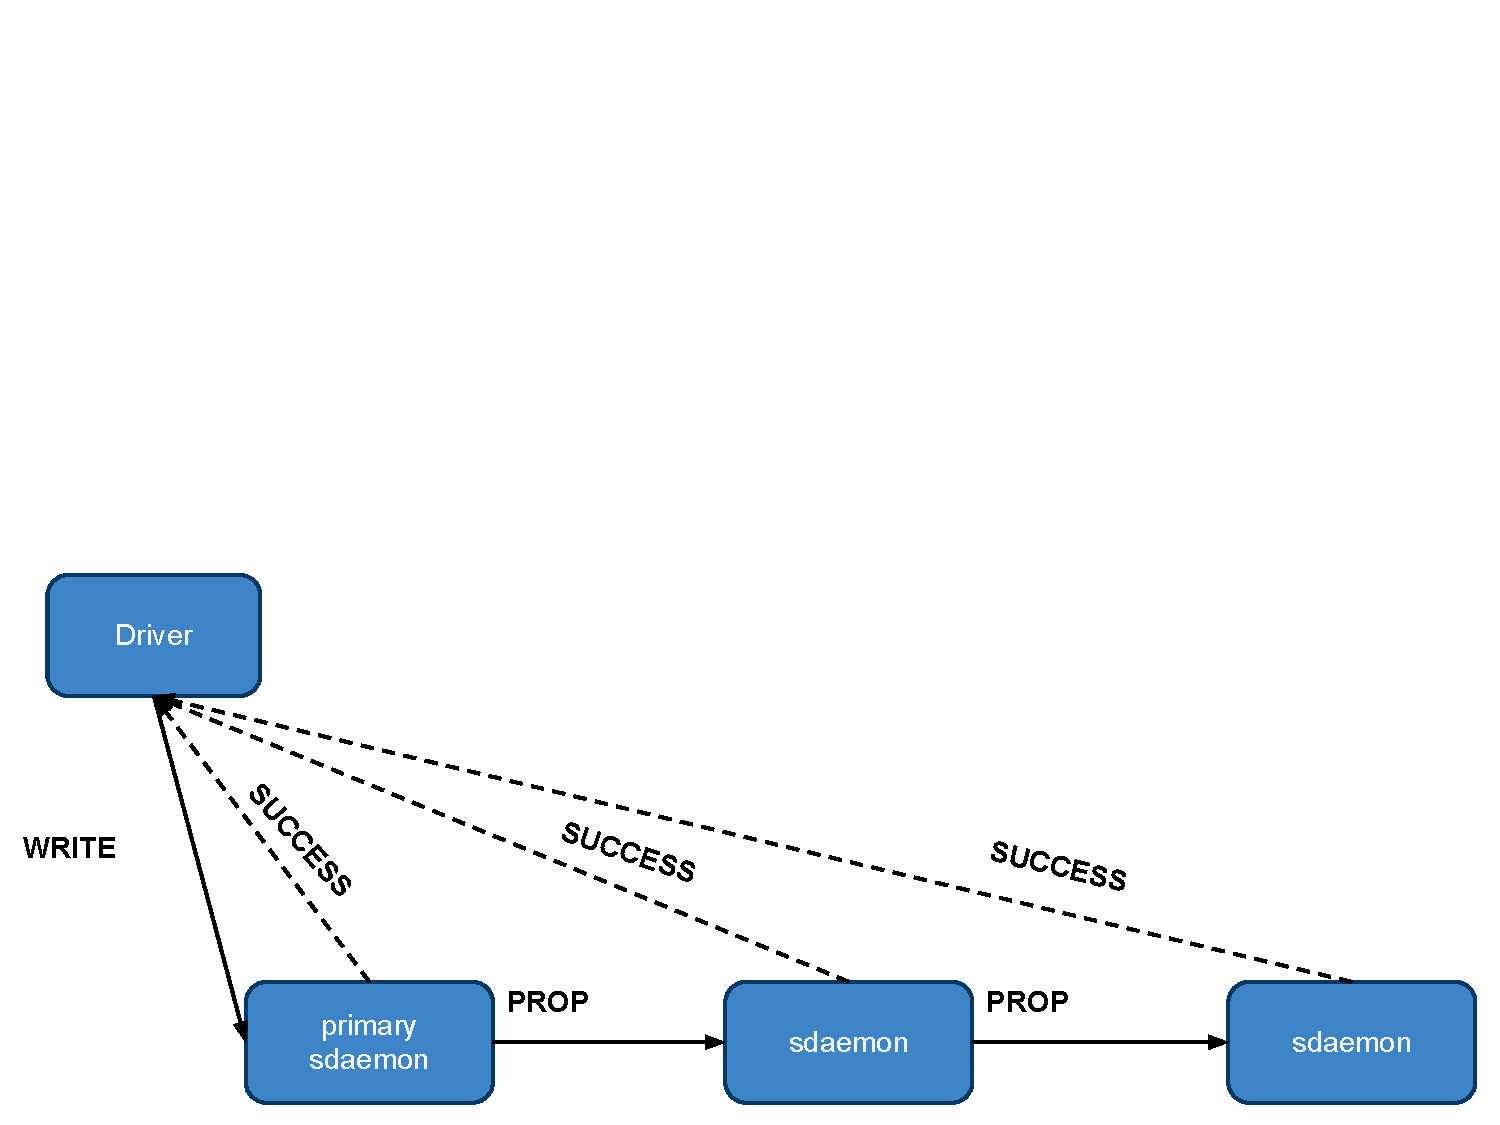
\includegraphics[width=\textwidth, trim=0 0 0 3.5in, clip]{./figures/write.pdf}
        \caption{The message flow for a write operation. A quorum of SUCCESS 
                 responses must be received for a successful write.}
        \label{fig:write}
    \end{subfigure}
    ~
    \begin{subfigure}{0.5\textwidth}
        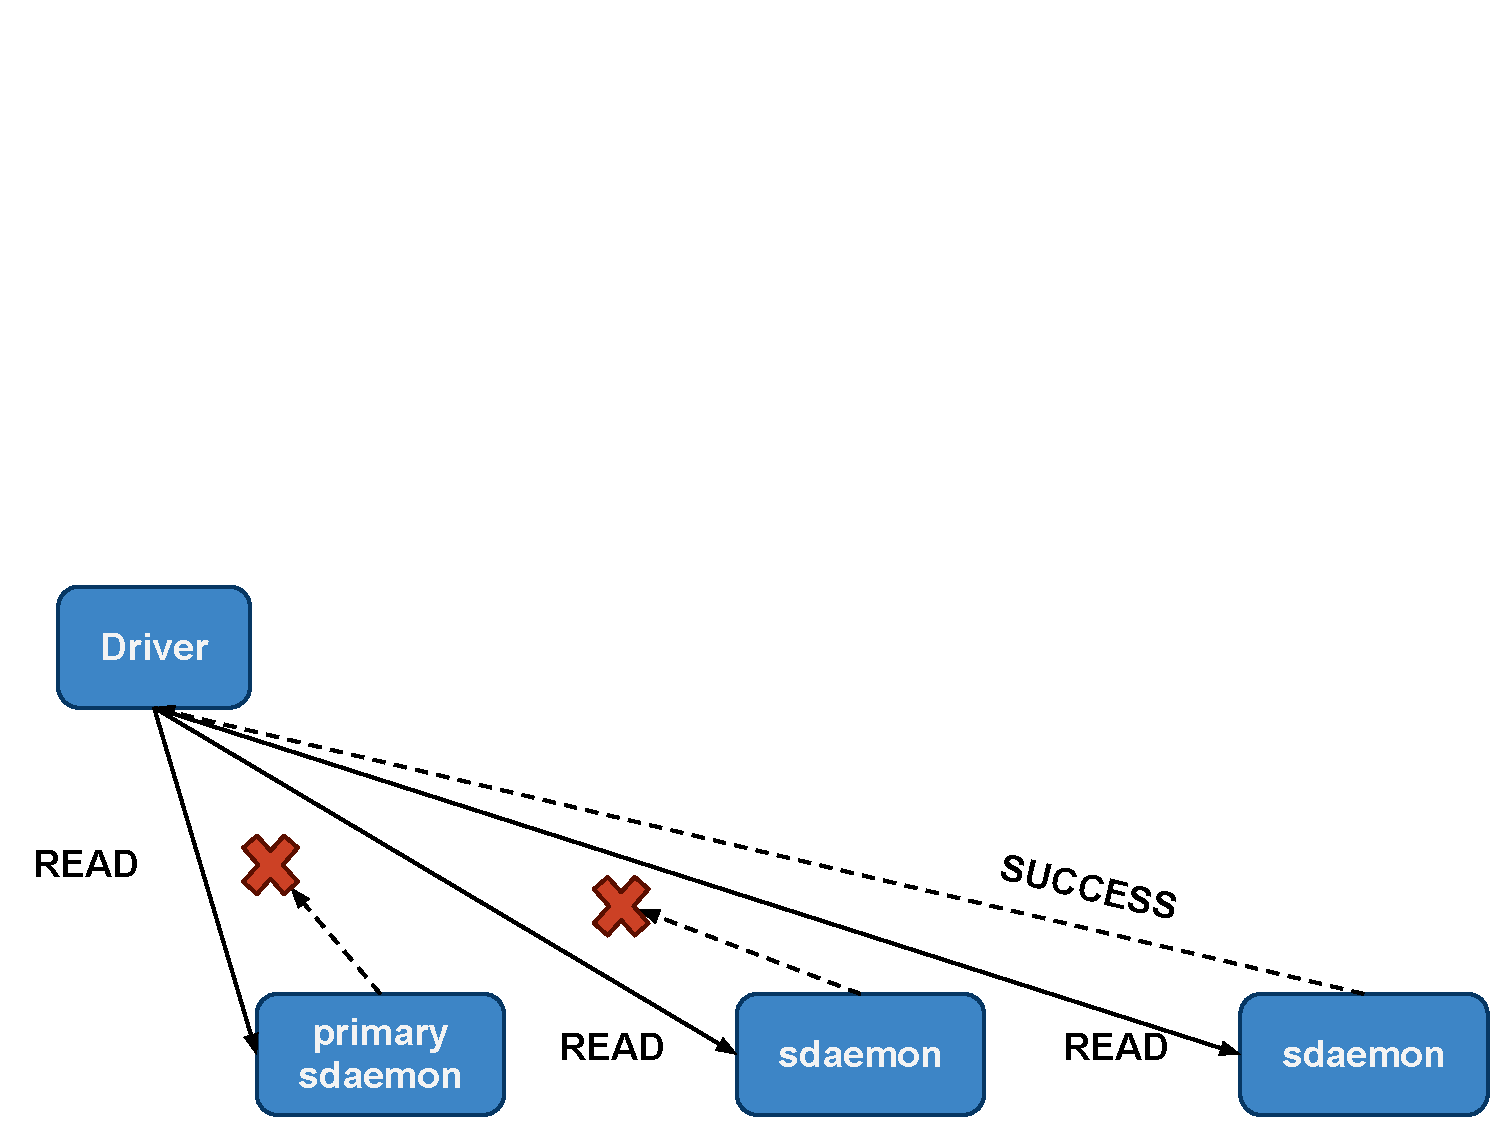
\includegraphics[width=\textwidth, trim=0 0 0 3.5in, clip]{./figures/read.pdf}
        \caption{The message flow for a read operation. A read request is 
            issued to the replica with the most recent version until a 
            SUCCESS is received or if no replicas with the most recent 
            version responds with SUCCESS.}
        \label{fig:read}
    \end{subfigure}
    \caption{Message flows for read and write operations}
\end{figure}

\subsection{Synchronization and Failure}
\label{sec:replication}
Replication is managed by \texttt{sdaemon} using write propagation and 
synchronization. Propagation was discussed in Section~\ref{sec:readwrite}. 
Synchronization is performed whenever a replica joins the chain and also 
periodically to keep replicas near the tail from becoming increasingly out 
of date. Figure~\ref{fig:sync} shows how replication is performed. As we see,
replica C sends a SYNC request with the version number of its local LSVD 
copy to the previous replica in the chain, replica B. Replica B then responds
with all the writes from C.version to B.version. Replica C then applies all 
the writes to its LSVD. After the synchronization operation, Replica C's 
LSVD version is equal to B.version. Similarly, replica B initiates the 
synchronization procedure with replica A.

To handle failure, a replica controller is used to inform the driver and 
neighboring replicas that a failure has occured. This controller keeps track 
of the liveliness of each replica by recording the elapsed time since the 
last heartbeat message, which is sent every $T$ seconds by each replica. 
After $4T$ seconds the replica is marked as failed. Upon failure, the 
controller informs the driver and the next replica server in the 
chain using update messages. Upon receipt of the update message, the 
successor replica connects to the replica ahead of the faulting server, which
updates its next server information. The successor replica then sends a SYNC 
request, and then normal operation resumes. Meanwhile, the controller spins 
off a new \texttt{sdaemon} process that is appended to the end of the chain. 
The driver appropriately modifies its replica version list by deleting the
faulted server and adding the new server and then connects to the new server
to retrieve its current version.
In order to minimize the amount of synchronization that needs to be 
performed on startup, we use a copy of the LSVD of the tail replica on 
initialization. In Section~\ref{sec:lsvd} we discuss how we handle LSVD
failure. Note that the replica controller is currently not 
implemented in our prototype. 

\begin{figure}[t]
    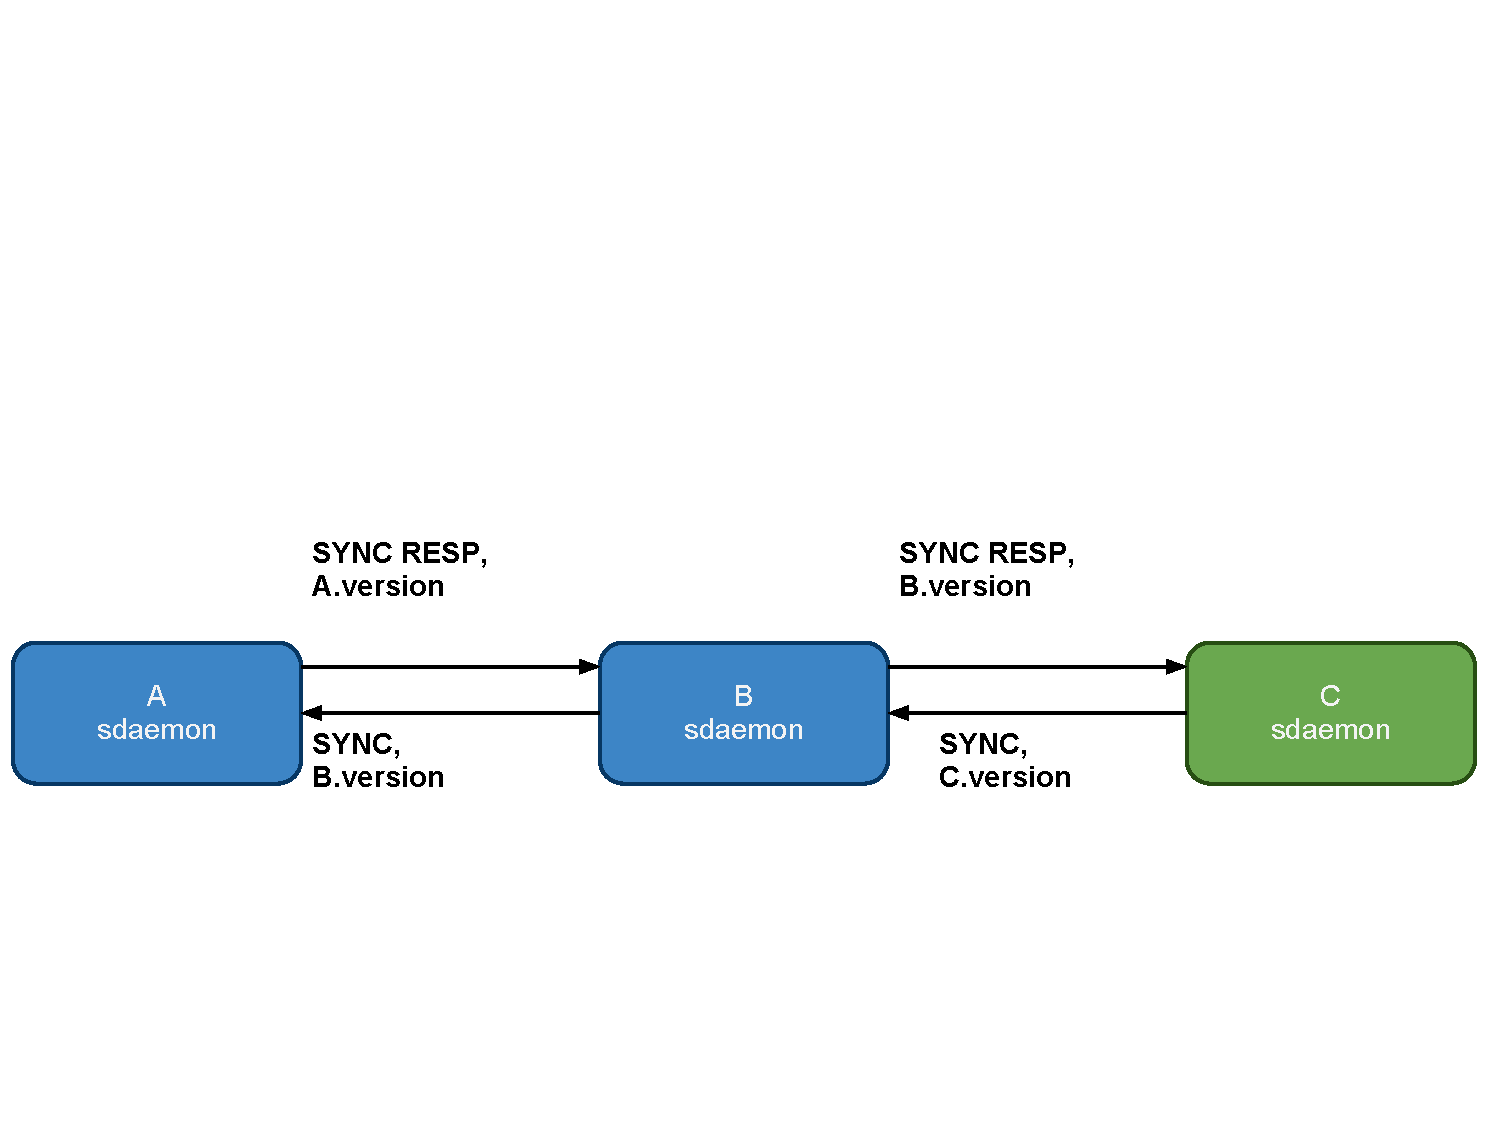
\includegraphics[width=0.45\textwidth, trim=0 2in 0 3in, clip]{./figures/sync.pdf}
    \caption{The message flow for a synchronization operation. Replica C 
            sends a SYNC request to its predecessor, which responds with all
            the writes since C's version.}
    \label{fig:sync}
\end{figure}

\subsection{Log Structured Virtual Disk}
\label{sec:lsvd}

When designing our file format to back virtual disk, we had few goals in mind. First, the file should be dynamically growing. If a disk is defined with $D$ bytes free space and the user only uses $C$ bytes for her content, the backing file size should use on the order of $O(C)$ bytes. Second, we must support versioning. We define $version$ as a monotonically increasing update sequence number. Each update increments the disk version by one. An update is a request originating from the driver that consists of one or more sequential sectors on the disk. Moreover, versions are required to enable synchronization; \texttt{sdaemon} must be aware of the current local disk version and must be able to send arbitrary version updates to other replicas for synchronization. The third goals for LSVD was consistency. If the local data has version $V$, it should consist of all updates with versions less than or equal to $V$ and no updates with versions greater than $V$. Finally, the fourth goal was the ability to easily support snapshots and incremental backups.

To address all of these requirements, we developed Log Structured Virtual Disk (LSVD). When LSVD receives updates, it writes them sequentially on the backing file and increments the LSVD version by one. This append-on-write behaviour, along with the LSVD cleanup procedure, satisfies our dynamically growing file goal. We also support versioning and consistentency by recording all modifications and their corresponding versions. When designing the LSVD, we took special care to ensure that the backing file remains consistent and recoverable up to a recent version, even if the replica server fails at any arbitrary point in time. Finally, LSVD provides the framework for snapshoting and incremental backups; however, this is not currently implemented. To extend LSVD for snapshot operation, we just create new file and use old file as a base. New updates go to the new file and we can read old data from old, read-only base file. \XXX{Extend this? Yes, please extend this. I don't understand how this is like the Amazon EBS snapshot? It sounds more like a full clone. Also, incremental backups? }

Figure \ref{fig:lsvd} shows the layout of an LSVD file. The first few bytes define the superblock, which contains important metadata\XXX{such as?}. Following this there are two checkpointing placeholders. After these we store the updates. Each update consists of a data block and a commit block. The data block is comprised of one or two sectors of write data. The commit block verifies the integrity of the data block by storing its checksum.\XXX{why do you need the checksum?} To guarantee consistency, we require atomic version writes; thus if a commit block is not written to disk or its checksum is invalid, we define the update as not committed and that update is skipped.

LSVD handles writes by appending the modified blocks to the end of the file with additional metadata. This means that sequential blocks may not exist in a contiguous layout on the physical disk. Therefore, on a read we use an in-memory \emph{sector to offset map} that maps LSVD disk sectors to their corresponding backing file offset. We update this mapping on every write. 


\begin{figure}[h]
    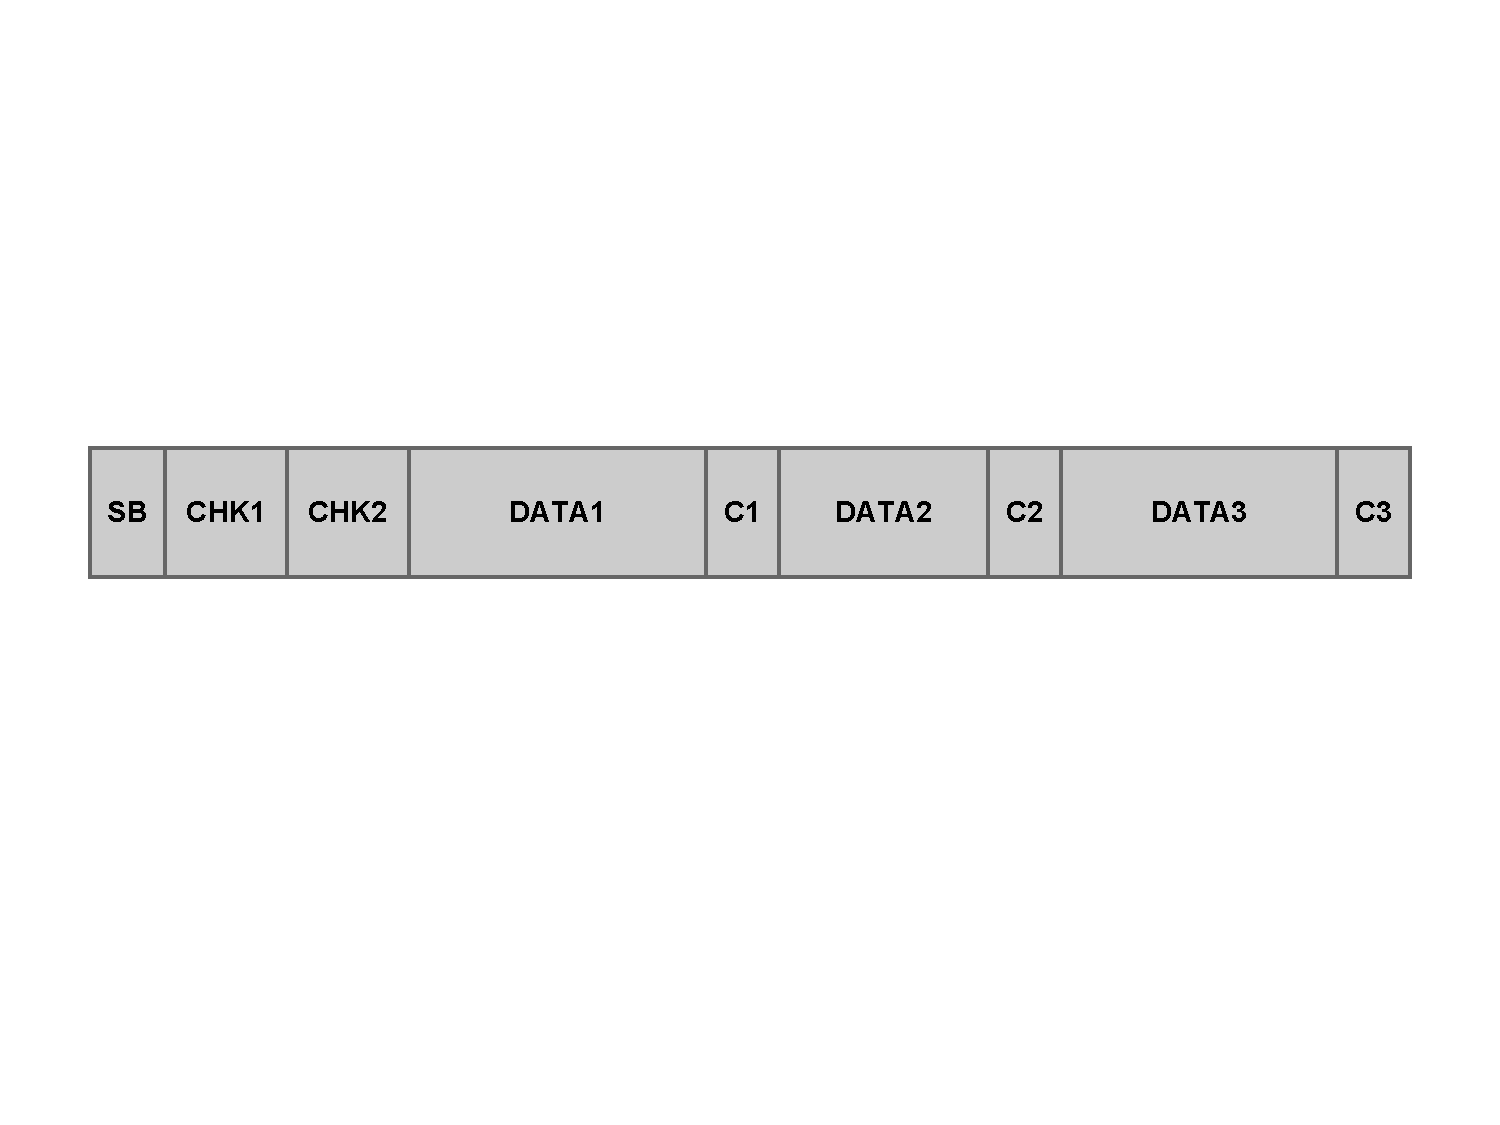
\includegraphics[width=0.45\textwidth]{./figures/lsvd.pdf}
    \caption{The LSVD file structure.}
    \label{fig:lsvd}
\end{figure}

\XXX{Probably could make this part its own subsubsection}
When opening a disk after recovery, LSVD could rebuild the sector to offset map by reading all the updates from the beginning of time; however, this method is slow. To keep recovery time from growing linearly with time, we perform \emph{checkpointing}. Every 60 seconds, we write the sector to offset map to disk into one of the checkpointing placeholders at the beginning of the file. In order to negate the impact of checkpoints on normal write or read operations, they are performed slowly. After a checkpoint is fully written to one of the placeholders, LSVD updates the superblock checkpoint pointer and calls \texttt{fsync} to flush the write to the physical disk. During recovery, the checkpoint data (sector to offset map) is loaded into memory and recovery continues from the point in time when checkpoint was started.\XXX{elaborate? what do you mean by "recoery continues from the point in time...? Do you replay updates?} By checkpointing periodically recovery time is correlated to the rate of updates rather than the total number of updates over time.

The problem with storing data in an append-on-write, log-structured format is data redundancy, or bloat. Even if a sector has been overwritten by newer data, LSVD still keeps its old versions around. This is both advantageous and disadvantageous. For instance, we can use it to enable users to recover the disk state from an arbitrary point in time. However, the file may grow to an unmanageable size. We therefore implement garbage collection with a goal of reclaiming state from sectors that have been overwritten with newer data. To do this, we developed a separate \texttt{cleanup} function that reads in an LSVD file and essentially flattens all updates into the latest version. The \texttt{cleanup} function does this by reading the file and reconstructing the sector to offset map. It then starts at the beginning of the file and considers all updates on the disk sequentially. If any of the sectors contained in the update is up-to-date, the update is appended to the new file. The process skips the update if all sectors were overwritten. Since the LSVD file is guaranteed to be consistent at any point in time, we can execute cleanup during live operation. Once the new file is constructed, it can be brought up-to-date with the replica synchronization protocol. After it has been synchronized, we can transparently change the backing file used by LSVD to the new, compacted version and delete the old file. We have not implemented the hot swap, however. Note that there are two drawbacks of this garbage collection approach. First, it must read and process the entire file, which can be a slow operation. Second, it requires enough free space on the current drive to store the new file. However, if we store $O(n)$ files on the disk and run cleanup on them in round robin fashion, we need free space for only $O(1)$ disks. \XXX{Elaborate? is this a partitioned file scheme?}

We implemented LSVD as a C library. Figure \ref{fig:lsvdinterface} shows the interface exposed by the library. Most of the functions are straight forward. We use functions \texttt{get\_writes\_lsvd} and \texttt{put\_writes\_lsvd} to support replica synchronization. \texttt{get\_writes\_lsvd} returns raw update data for all updates since \texttt{first\_version}. We do not keep a version to offset map, so we must scan all the updates backwards until we encounter a version less than or equal to \texttt{first\_version}. Once we find the requested starting version, we copy the raw update data into the buffer. The raw data is then transferred to the lagging replica and appended to its LSVD file using function \texttt{put\_writes\_lsvd}, bringing it up-to-date.

\lstset{language=C}
\lstset{basicstyle=\small}
\lstset{frame=tlrb}
\begin{figure}
\begin{lstlisting}
struct lsvd_disk *create_lsvd(
	const char *pathname, uint64_t size);
struct lsvd_disk *open_lsvd(
	const char *pathname);
int cleanup_lsvd(const char *old_pathname, 
	const char *new_pathname);
int read_lsvd(struct lsvd_disk *lsvd,
	char *buf, uint64_t length,
	uint64_t offset, uint64_t version);
int write_lsvd(struct lsvd_disk *lsvd,
	const char *buf, uint64_t length, 
	uint64_t offset, uint64_t version);
int fsync_lsvd(struct lsvd_disk *lsvd);
uint64_t get_version(struct lsvd_disk *lsvd);
char *get_writes_lsvd(struct lsvd_disk *lsvd, 
	uint64_t first_version, size_t *size);
int put_writes_lsvd(struct lsvd_disk *lsvd, 
	uint64_t first_version, char *buf,
	size_t size);
int close_lsvd(struct lsvd_disk *lsvd);
\end{lstlisting}
\caption{LSVD library interface}
\label{fig:lsvdinterface}
\end{figure}
